\documentclass{article}
\usepackage{ae,aecompl}
\usepackage{todonotes}
\usepackage{chngcntr}
\usepackage{tikz-cd}
\usepackage{graphicx}
\graphicspath{ {./images/}}
\usepackage[all,cmtip]{xy}
\usepackage{amsmath, amscd}
\usepackage{amsthm}
\usepackage{amssymb}
\usepackage{amsfonts}
\usepackage{bm}
\usepackage{qsymbols}
\usepackage{latexsym}
\usepackage{mathrsfs}
\usepackage{mathtools}
\usepackage{cite}
\usepackage{color}
\usepackage{url}
\usepackage{enumerate}
\usepackage{verbatim}
\usepackage[draft=false, colorlinks=true]{hyperref}
\usepackage{pdfpages}
\usepackage[margin=1.2in]{geometry}
\usepackage{IEEEtrantools}

\usepackage{fancyhdr}


\usepackage[nameinlink]{cleveref}


\DeclareMathOperator*{\ac}{accept}
\DeclareMathOperator*{\amax}{argmax}
\DeclareMathOperator*{\amin}{argmin}
\DeclareMathOperator*{\Aut}{Aut}
\newcommand {\al}{{\alpha}}
\newcommand {\abs}[1]{{\left\lvert#1\right\rvert}}
\newcommand {\A}{{\mathcal{A}}}
\newcommand {\AM}{{\mathrm{AM}}}
\newcommand {\AMp}{{\AM_{p}^{X}\!(\Ri_\w)}}
\newcommand {\B}{{\mathcal{B}}}
\DeclareMathOperator*{\Be}{Bern}
\newcommand {\Br}{{\dot{B}}}
\newcommand {\Ba}{{\mathfrak{B}}}
\newcommand {\C}{{\mathbb C}}
\newcommand {\ce}{\mathrm{c}}
\newcommand {\Ce}{\mathrm{C}}
\newcommand {\Cc}{\mathrm{C_{c}}}
\newcommand {\Ccinf}{\mathrm{C_{c}^{\infty}}}
\DeclareMathOperator{\cov}{Cov}
\DeclareMathOperator{\DEV}{DEV}
\newcommand {\Di}{{\mathbb D}}
\newcommand {\dom}{\mathrm{dom}}
\newcommand{\dist}{\stackrel{\mathrm{dist}}{=}}
\newcommand {\ud}{\mathrm{d}}
\newcommand {\ue}{\mathrm{e}}
\newcommand {\eps}{\varepsilon}
\newcommand {\veps}{\varepsilon}
\newcommand {\vrho}{{\varrho}}
\newcommand {\E}{{\mathbb{E}}}
\newcommand {\Ec}{{\mathcal{E}}}
\newcommand {\Ell}{L}
\newcommand {\Ellp}{{L_{p}[0,1]}}
\newcommand {\Ellpprime}{{L_{p'}([0,1])}}
\newcommand {\Ellq}{{L_{q}([0,1])}}
\newcommand {\Ellqprime}{{L_{q'}([0,1])}}
\newcommand {\Ellr}{L^{r}}
\newcommand {\Ellone}{{L_{1}([0,1])}}
\newcommand{\Elltwo}{{L_{2}([0,1])}}
\newcommand{\Ellinfty}{L^{\infty}}
\newcommand{\Ellinftyc}{L_{\mathrm{c}}^{\infty}}
\newcommand{\exb}[1]{\exp\left\{#1\right\}}
\DeclareMathOperator*{\Ext}{Ext}
\newcommand{\F}{{\mathcal{F}}}
\newcommand{\Fe}{{\mathbb{F}}}
\newcommand{\G}{{\mathcal{G}}}
\newcommand{\HF}{\mathcal{H}_{\text{FIO}}^{1}(\Rd)}
\newcommand{\Hr}{H}
\newcommand{\HT}{\mathcal{H}}
\newcommand{\ui}{\mathrm{i}}
\newcommand{\I}{{I}}
\newcommand{\J}{{\mathcal{J}}}
\newcommand{\id}{{\mathrm{id}}}
\newcommand{\iid}{\stackrel{\mathclap{\normalfont\mbox{iid}}}{\sim}}
\newcommand{\im}{{\text{im }}}
\newcommand{\ind}{{\perp\!\!\!\perp}}
\DeclareMathOperator*{\Int}{int}
\newcommand{\intx}{{\overline{\int_{X}}}}
\newcommand{\inte}{{\overline{\int_{\E}}}}
\newcommand{\la}{\lambda}
\newcommand{\rb}{\rangle}
\newcommand{\lb}{{\langle}}
\newcommand{\La}{\Lambda}
\newcommand{\calL}{{\mathcal{L}}}
\newcommand{\lp}{{\mathcal{L}}^{p}}
\newcommand{\lpo}{{\overline{\mathcal{L}}^{p}\!}}
\newcommand{\Lpo}{{\overline{\Ell}^{p}\!}}
\newcommand{\M}{{\mathbf{M}}}
\newcommand{\Ma}{{\mathcal{M}}}
\newcommand{\N}{{{\mathbb N}}}
\newcommand{\Na}{{{\mathcal{N}}}}
\newcommand{\norm}[1]{\left\|#1\right\|}
\newcommand{\normm}[1]{{\left\vert\kern-0.25ex\left\vert\kern-0.25ex\left\vert #1 
    \right\vert\kern-0.25ex\right\vert\kern-0.25ex\right\vert}}
\newcommand{\Om}{{{\Omega}}}
\newcommand{\one}{{{\bf 1}}}
\newcommand{\pic}{\text{Pic }}
\newcommand{\ph}{{\varphi}}
\newcommand{\Pa}{{\mathbb{P}}}
\newcommand{\Po}{{\mathcal{P}}}
\newcommand{\Q}{{\mathbb{Q}}}
\newcommand{\R}{{\mathbb R}}
\newcommand{\Rd}{{\mathbb{R}^{d}}}
\DeclareMathOperator{\rej}{reject }
\newcommand{\Rn}{{\mathbb{R}^{n}}}
\newcommand{\cR}{{\mathcal{R}}}
\newcommand{\Rad}{{\mathrm{Rad}}}
\newcommand{\ran}{{\mathrm{ran}}}
\newcommand{\Ri}{{\mathrm{R}}}
\newcommand{\supp}{{\mathrm{supp}}}
\newcommand{\Se}{\mathrm{S}}
\newcommand{\Sp}{S^{*}(\Rn)}
\newcommand{\St}{{\mathrm{St}}}
\newcommand{\Sw}{\mathcal{S}}
\newcommand{\T}{{\mathcal{T}}}
\newcommand{\ta}{{\theta}}
\newcommand{\Ta}{{\Theta}}
\newcommand{\topp}{\stackrel{p}{\to}}
\newcommand{\todd}{\stackrel{d}{\to}}
\newcommand{\toL}[1]{\stackrel{L^{#1}}{\to}} 
\newcommand{\toas}{\stackrel{a.s.}{\to}}
\DeclareMathOperator{\V}{Var}
\newcommand {\w}{{\omega}}
\newcommand {\W}{{\mathrm{W}}}
\newcommand {\Wnp}{\text{$\mathrm{W}$\textsuperscript{$n,\!p$}}}
\newcommand {\Wnpeq}{\text{$\mathrm{W}$\textsuperscript{$n\!,\!p$}}}
\newcommand {\Wonep}{\text{$\mathrm{W}$\textsuperscript{$1,\!p$}}}
\newcommand {\Wonepeq}{\text{$\mathrm{W}$\textsuperscript{$1\!,\!p$}}}
\newcommand {\X}{{\mathcal{X}}}
\newcommand {\Z}{{{\mathbb Z}}}
\newcommand {\Za}{{\mathcal{Z}}}
\newcommand {\Zd}{{\Z[\sqrt{d}]}}
\newcommand {\vanish}[1]{\relax}

\newcommand {\wh}{\widehat}
\newcommand {\wt}{\widetilde}
\newcommand {\red}{\color{red}}

% Distributions
\newcommand{\normal}{\mathsf{N}}
\newcommand{\poi}{\mathsf{Poisson}}
\newcommand{\bern}{\mathsf{Bernoulli}}
\newcommand{\bin}{\mathsf{Binomal}}
\newcommand{\multi}{\mathsf{Multinomial}}
\newcommand{\Exp}{\mathsf{Exp}}



% put your command and environment definitions here




% some theorem environments
% remove "[theorem]" if you do not want them to use the same number sequence


  \newtheorem{thrm}{Theorem}
  \newtheorem{lemma}{Lemma}
  \newtheorem{prop}{Proposition}
  \newtheorem{cor}{Corollary}

  \newtheorem{conj}{Conjecture}
  \renewcommand{\theconj}{\Alph{conj}}  % numbered A, B, C etc

  \theoremstyle{definition}
  \newtheorem{defn}{Definition}
  \newtheorem{ex}{Example}
  \newtheorem{exs}{Examples}
  \newtheorem{question}{Question}
  \newtheorem{remark}{Remark}
  \newtheorem{notn}{Notation}
  \newtheorem{exer}{Exercise}




\title{STATS305A - Lecture 19}
\author{John Duchi\\ Scribed by Michael Howes}
\date{12/02/21}

\pagestyle{fancy}
\fancyhf{}
\rhead{STATS305A - Lecture 19}
\lhead{12/02/21}
\rfoot{Page \thepage}

\begin{document}
\maketitle
\tableofcontents
\section{Announcements}
Final homework and etude are avialable on the website.
\section{Predictive inference}
\subsection{Setting and motivation}
Given data $(X_i,Y_i)_{i=1}^n$ we would like to find a confidence set mapping $\wh{C}:\X \to \ell$ where $\X$ is the space of $X$ and $\ell = \{[a,b]: a\le b\}$ is the set of all intervals in $\R$. We would want the confidence set mapping $\wh{C}$ to have the property that if we have a new sample $(X_{n+1},Y_{n+1})$, then $Y_{n+1} \in \wh{C}(X_{n+1})$ some prescribed high probability i.e. above some threshold $1-\al$. 

There are two ways we can formalize this property:
\begin{enumerate}
    \item We could ask for \emph{conditional coverage} (CC). That is we want a procedure $\wh{C}$ that satisfies 
    \[\Pa(Y_{n+1} \in \wh{C}(x)|X_{n+1}=x) \ge 1-\al,\] for (almost) all $x \in \X$. Unfortunately this is not possible as shown by Vovk/Lei \& Wasserman: If the procedure $\wh{C}$ satisfies (CC) for all $\Pa$, then $\E[\text{length}(\wh{C}(x))]=+\infty$ for almost all $x \in \X$ that are not atoms of $\Pa$. 
    \item We can achieve \emph{marginal coverage}. That is we can achieve CC on average over $x$. We will see a procedure $\wh{C}$ which is a function of $(X_i,Y_i)_{i=1}^n \iid \Pa$ such that 
    \[\Pa(Y_{n+1}\in \wh{C}(X_{n+1})) \ge 1-\al. \]
    The procedure we will describe is distribution \underline{and} model independent and very general. The procedure can be viewed as a protective wrapper around any black box model that will still guarantee coverage and validty. The basic idea is that we will construct confidence sets to evaluate the ``weirdness'' of new data $Y_{n+1}$.
\end{enumerate}
\section{Permutations, qunatiles and p-values}
Suppose that $(Z_i)_{i=1}^n$ are exchangeable. That is 
\[(Z_i)_{i=1}^n \stackrel{\text{dist}}{=} (Z_{\pi(i)})_{i=1}^n, \]
for all permuations $\pi$. Let $Z_{(1)}\le Z_{(2)} \le\ldots\le Z_{(n)}$ be the order statistics of $Z_i$. Recall that we previously define the emperical CDF $F_n(t)$ to be the function 
\[F_n(t) = \frac{1}{n}\sum_{i=1}^n \one(Z_i \le t). \]
The emperical CDF looks something like the below blue curve:
\begin{center}
    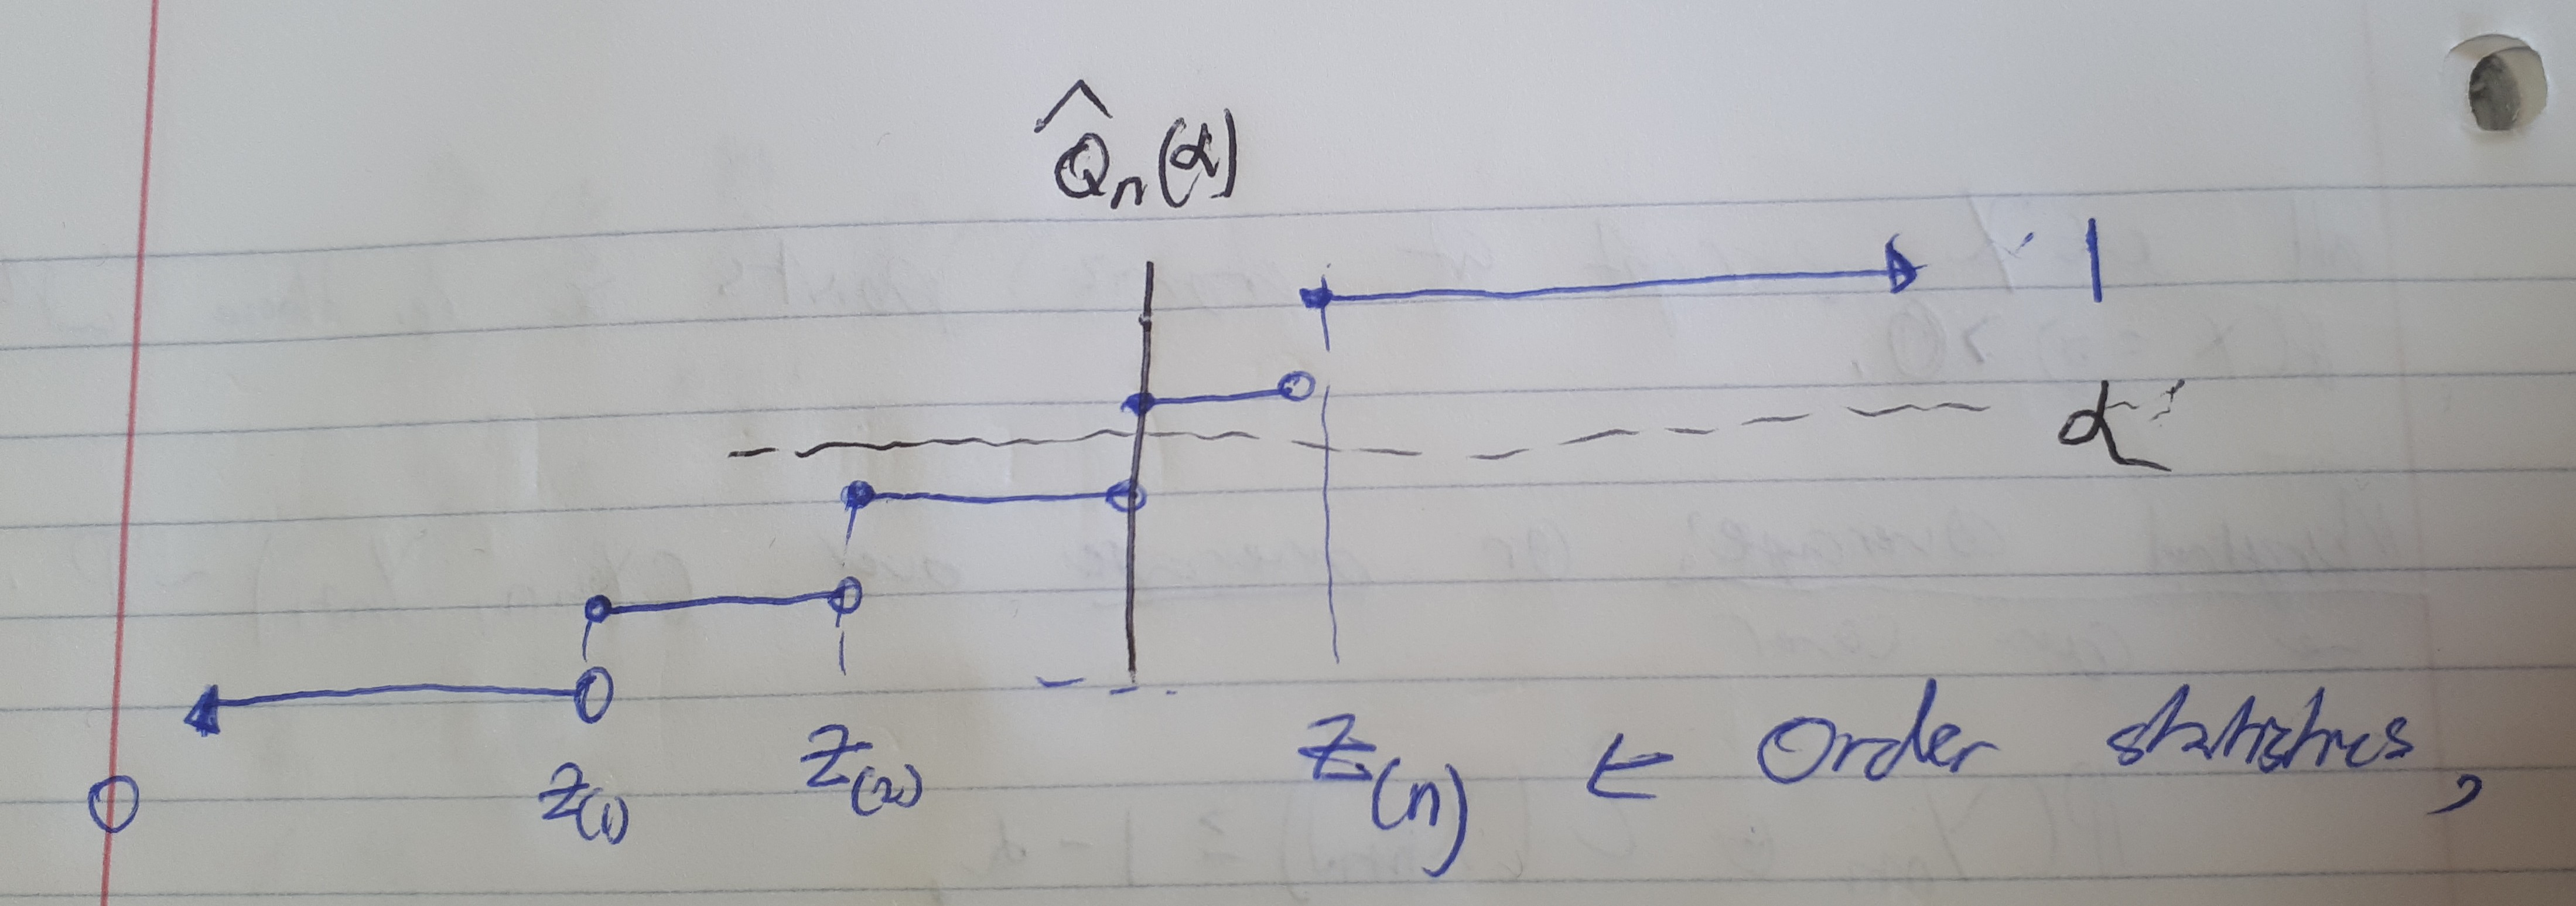
\includegraphics[width = 0.7\textwidth]{12_02_P01.jpg}
\end{center}
We also defined the quantile function $\wh{Q}_n(\al)$ given by 
\[\wh{Q}_n(\al) = \inf\{t \in \R : F_n(t)\ge \al\} = Z_{(\lceil \al n \rceil)}. \]
The quantile function $\wh{Q}_n$ is also illustrated in the above picture. When studying permutation tests we proved the below lemma.
\begin{lemma}
    If $(Z_i)_{i=1}^n$ are exchangeable, then 
    \[\Pa(Z_n \le \wh{Q}_n(\al))\ge \al. \]
    Likewise, if $Z_i$ are distinct with probablity 1, then 
    \[\Pa(Z_n \le \wh{Q}_n(\al))\le \al-\frac{1}{n}. \]
\end{lemma}
What is we want to add a new point $Z_{n+1}$. Suppose now that $(Z_i)_{i=1}^{n+1}$ are exchangeable. Can we use $(Z_i)_{i=1}^n$ to measure how ``weird'' $Z_{n+1}$ is?
\begin{notn}
    Let $Z_{(i,n)}$ be the order statistics of $(Z_i)_{i=1}^n$ and let $Z_{(i,n+1)}$ be the order statistics of $(Z_i)_{i=1}^{n+1}$.
\end{notn}
\begin{lemma}
    Let $k \in \{1,\ldots,n\}$, then 
    \[Z_{n+1} \le Z_{(k,n)} \Longleftrightarrow Z_{n+1} \le Z_{(k,n+1)}. \]
\end{lemma}
\begin{proof}
    First suppose that $Z_{n+1} \le Z_{(k,n)}$. Our order statistics thus look something like this:
    \begin{center}
        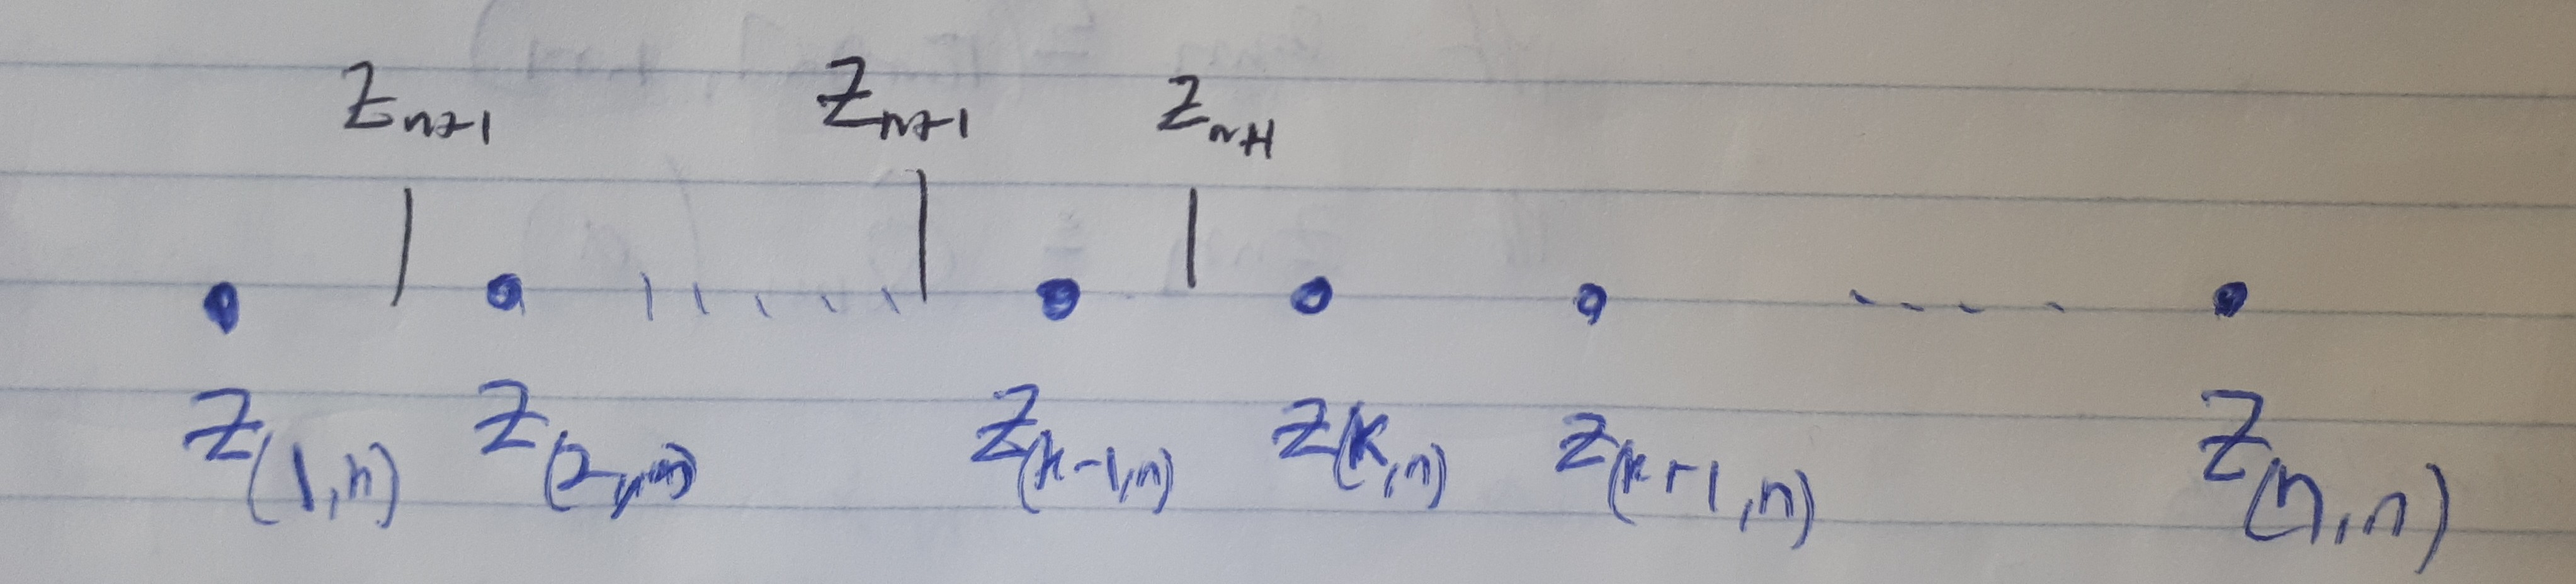
\includegraphics[width = 0.7\textwidth]{12_02_P02.jpg}
    \end{center}
    We will now consider two cases. If $Z_{n+1} \le Z_{(k-1,n)}$, then $Z_{(k,n+1)}=Z_{(k-1,n)}$. On the other hand if $Z_{n+1} > Z_{(k-1,n)}$, then $Z_{(k,n+1)}=Z_{n+1}$. Thus we have
    \[Z_{(k,n+1)} = \max\{Z_{n+1}, Z_{(k-1,n)}\}. \]
    Therefore $Z_{n+1} \le Z_{(k,n+1)}$.

    Now conversely suppose that $Z_{n+1} \le Z_{(k,n+1)}$. We always have $Z_{(k,n+1)} \le Z_{(k,n)}$. We can thus conclude that $Z_{n+1}\le Z_{(k,n)}$.
\end{proof}
\begin{cor}
    Suppose $(Z_i)_{i=1}^{n+1}$ are exchangeable. For any $\al \in [0,1]$,
    \[\Pa\left(Z_{n+1} \le \wh{Q}_n\left(\frac{n+1}{n}\al\right)\right) \ge \al.\]
    Furthermore if $(Z_i)_{i=1}^{n+1}$ are distinct with probability 1, then 
    \[\Pa\left(Z_{n+1} \le \wh{Q}_n\left(\frac{n+1}{n}\al\right)\right) \le \al+\frac{1}{n+1}.\]
\end{cor}
\begin{proof}
    Note that 
    \[\wh{Q}_n\left(\frac{n+1}{n}\al\right)=Z_{\left(\left\lceil n\frac{n+1}{n} \al \right\rceil,n\right)}=Z_{\left(\left\lceil (n+1) \al \right\rceil,n\right)}.\]
    Thus
    \begin{align*}
        Z_{n+1}  \le \wh{Q}_n\left(\frac{n+1}{n}\al\right)&\Longleftrightarrow Z_{n+1} \le Z_{(\lceil (n+1)\al\rceil,n)}\\
        &\Longleftrightarrow Z_{n+1}\le Z_{(\lceil (n+1)\al\rceil,n+1)}\\
        &\Longleftrightarrow Z_{n+1}\le \wh{Q}_{n+1}(\al).
    \end{align*}
    Thus the result follows from Lemma 1.
\end{proof}
This corollary implies that 
\[\Pa\left(Z_{n+1} > \wh{Q}_n\left(\frac{n+1}{n}(1-\al)\right)\right) \le \al, \]
and if $(Z_i)_{i=1}^{n+1}$ are distinct with probability one, then 
\[\Pa\left(Z_{n+1} > \wh{Q}_n\left(\frac{n+1}{n}(1-\al)\right)\right) \ge \al-\frac{1}{n+1}. \]
\section{Split conformal inference}
How can we use these quantile ideas to make confidence intervals? Suppose that we have a model $\wh{f} : \X \to \R$ fitted on training data. Suppose also that we have validation data in the form of an i.i.d. sample $(X_i,Y_i)_{i=1}^n$ that is independent of $\wh{f}$. In practice this means splitting our data like so:
\begin{center}
    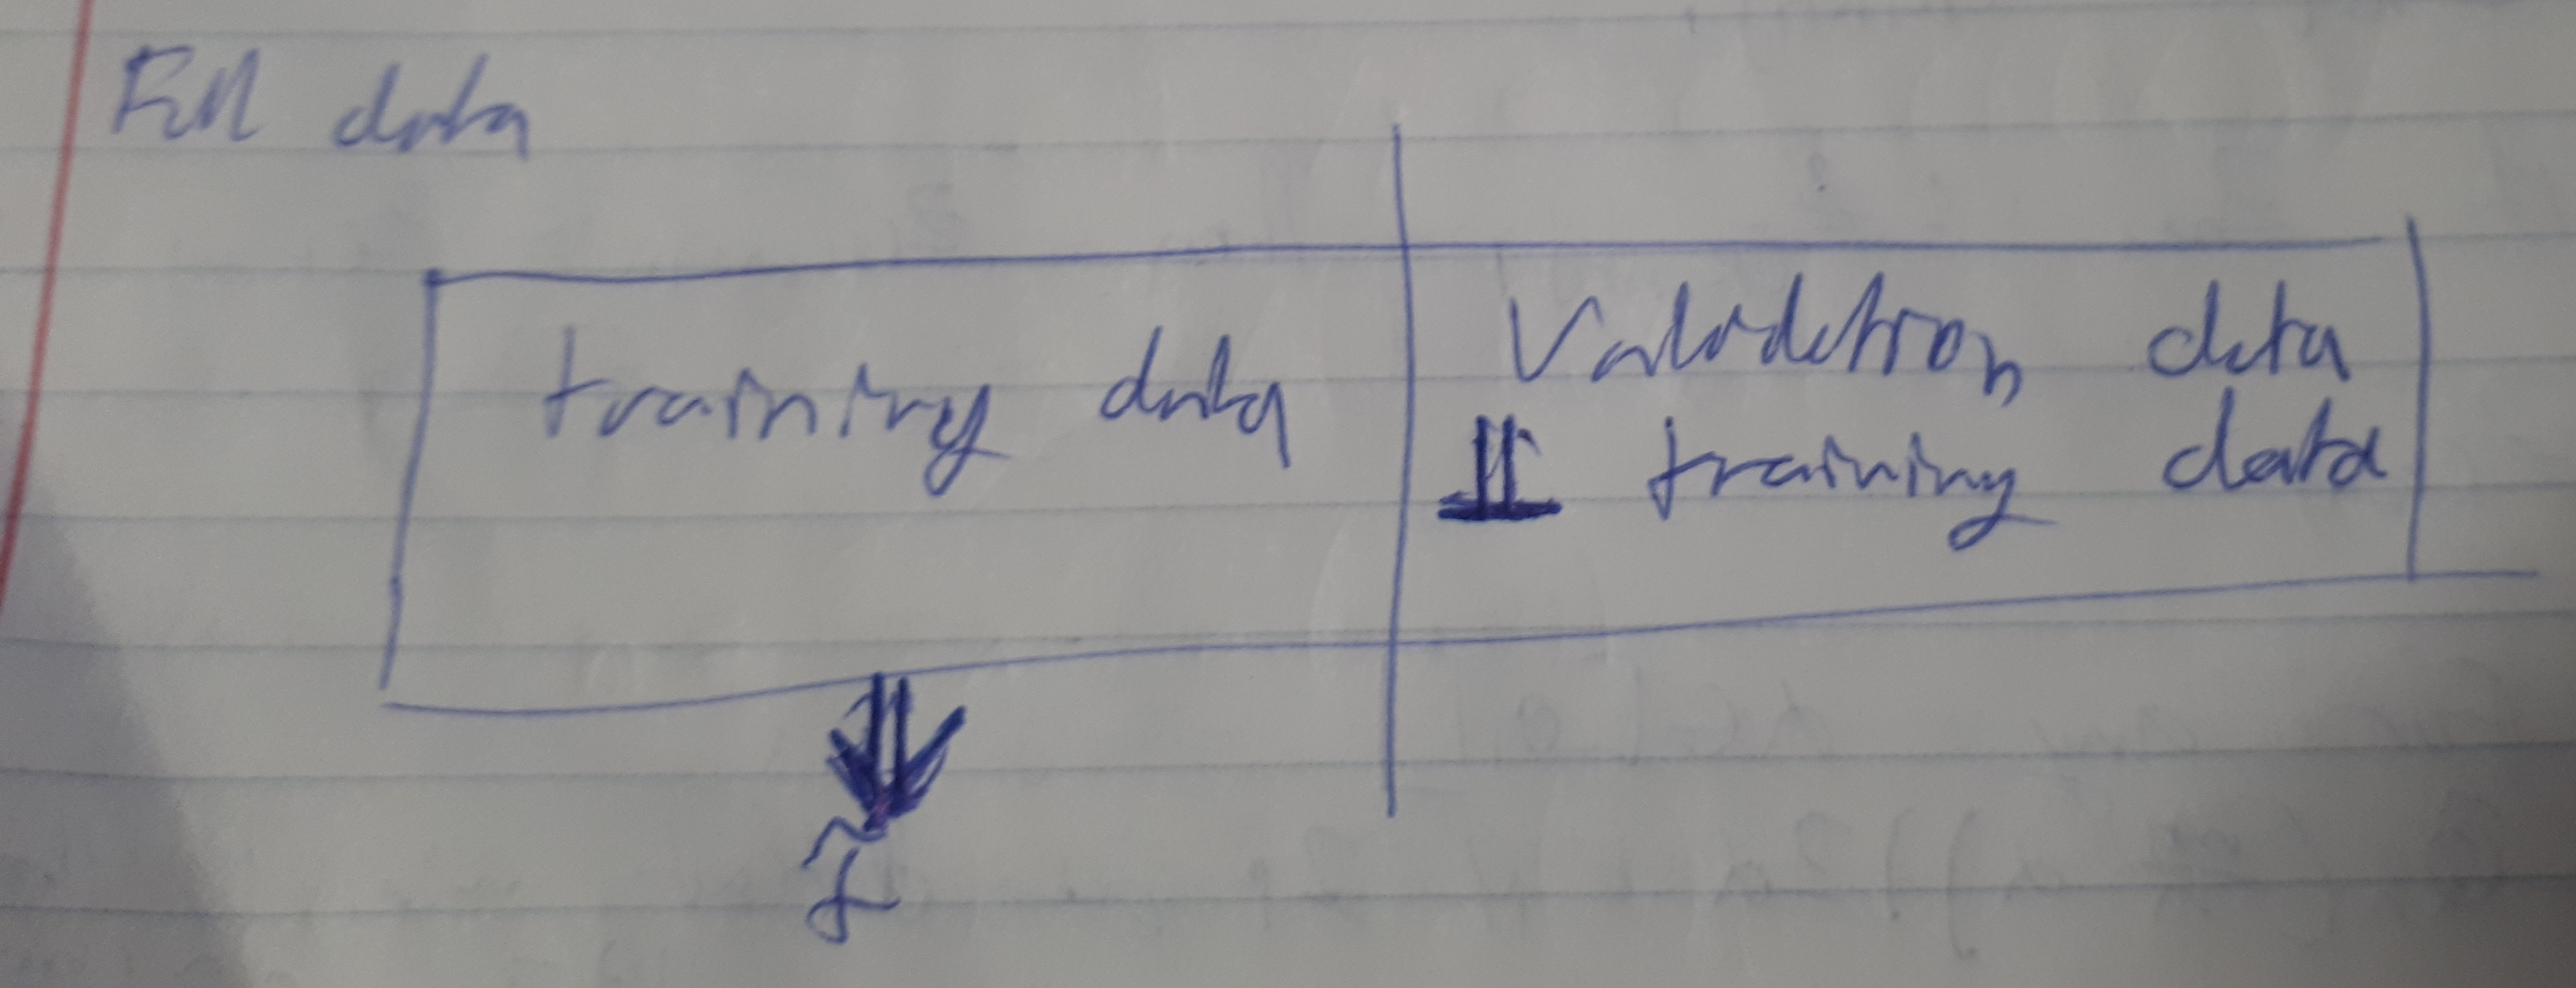
\includegraphics[width = 0.7\textwidth]{12_02_P03.jpg}
\end{center}
We will use the validation set $(X_i,Y_i)_{i=1}^n$ to find a valid confidence set. For each $i$ define $Z_i = \abs{Y_i-\wh{f}(X_i)}$ to be the \emph{non-conformity score} of $(X_i,Y_i)$. We can let $\wh{Q}_n$ be the quantile function for $(Z_i)_{i=1}^n$. Then on a new data point $(X_{n+1},Y_{n+1})$ we will have 
\[\Pa\left(Z_{n+1} > \wh{Q}_n\left(\frac{n+1}{n}(1-\al)\right)\right) \le \al. \]
How do we transform this into a confidence set? For $x \in \X$ and $\tau \ge 0$ define 
\[C_\tau(x):= [\wh{f}(x)-\tau, \wh{f}(x)+\tau].  \]
Then 
\[y \in C_\tau(x) \Longleftrightarrow y \in[\wh{f}(x)\pm \tau] \Longleftrightarrow \abs{\wh{f}(x)-y} \le \tau. \]
For a given $\al\in [0,1]$, take
\[\wh{\tau}_n = \wh{Q}_n\left(\frac{n+1}{n}(1-\al)\right), \]
and define $\wh{C}(x)=C_{\wh{\tau}_n}(x)$.
\begin{prop}
    With $\wh{C}$ as above we have 
    \[\Pa(Y_{n+1} \in \wh{C}(X_{n+1})) \ge 1-\al. \]
    Furthermore if $Z_i=\abs{Y_i-\wh{f}(X_i)}$ are distinct with probability 1, then 
    \[\Pa(Y_{n+1} \in \wh{C}(X_{n+1})) \le 1-\al+\frac{1}{n+1}. \]
\end{prop}
\begin{proof}
    We have already proven all of the main ingredients. Note that
    \begin{align*}
        Y_{n+1} \in \wh{C}(X_{n+1}) & \Longleftrightarrow \abs{\wh{f}(X_{n+1})-Y_{n+1}} \le \wh{\tau}_n\\
        &\Longleftrightarrow Z_{n+1} \le \wh{\tau}_n\\
        &\Longleftrightarrow Z_{n+1} \le \wh{Q}_n\left(\frac{n+1}{n}(1-\al)\right).
    \end{align*}
    Thus the result follows from Lemma 2.
\end{proof}
\begin{remark}
    We are getting confience sets for $Y_{n+1}$ not for $\E[Y_{n+1}|X_{n+1}]$ or anything like that. Note that the size of $\wh{C}(X)$ depends on how well the model $\wh{f}(X)$ performs on the independent validation set $(X_i,Y_i)_{i=1}^n$.
\end{remark}
\subsection{A general recipe}
We could have chosen lots of things other that $\abs{\wh{f}(X_i)-Y_i}$ for our conformal score $Z_i$. Here is one very general approach for creating conformal scores.

Suppose that our $Y$ now live in an arbitrary space $\mathcal{Y}$ and that we have a nested collection of confidence sets indexed by $\tau \in \R$. That is for each $\tau \in \R$ and $x \in \X$ we have a subset $C_\tau(x) \subseteq \mathcal{Y}$ such that for all $\tau_0 \le \tau_1$ and all $x \in \X$ we have
\[C_{\tau_0}(x) \subseteq C_{\tau_1}(x). \]
\begin{ex}
    Our previous choice of $C_\tau(x)$ was $C_\tau(x)=[\wh{f}(x)-\tau, \wh{f}(x)+\tau]$ which are indeed nested.
\end{ex}
We can use the collection $C_\tau(x)$ to define confidence scores $Z_i$ by
\[Z_i = \inf\{t\in \R : Y_i \in C_t(X_i)\}. \]
\begin{ex}
    If $C_\tau(x)=[\wh{f}(x)-\tau, \wh{f}(x)+\tau]$, then
    \[\inf\{t\in \R : Y_i \in C_t(X_i)\} = \abs{Y_i-\wh{f}(X_i)}, \]
    which matches the previous section.
\end{ex}
Define $\wh{Q}_n$ on $(Z_i)_{i=1}^n$ and let $\wh{\tau}_n = \wh{Q}_n\left(\frac{n+1}{n}(1-\al)\right)$. Then, as before, define
\[\wh{C}(x):= C_{\wh{\tau}_n}(x). \]
\begin{thrm}
    With $\wh{C}$ as above
    \[\Pa(Y_{n+1}\in \wh{C}(X_{n+1})) \ge 1-\al.\]
\end{thrm}
\begin{proof}
    Note that
    \begin{align*}
        Y_{n+1} \in \wh{C}(X_{n+1})&\Longleftrightarrow Y_{n+1} \in C_{\wh{\tau}_n}(X_{n+1})\\
        &\Longleftrightarrow Z_{n+1} \le \wh{\tau}_n \\
        & \Longleftrightarrow Z_{n+1} \le \wh{Q}_n\left(\frac{n+1}{n}(1-\al)\right) \qedhere
    \end{align*}
\end{proof}
\begin{ex}
    If $\mathcal{Y}$ is a metric space with metric $d$, then we can define 
    \[C_\tau(x) = \{y \in \mathcal{Y} : d(y,\wh{f}(x)) \le \tau\}, \]
    where $\wh{f}$ is some predictor trained on data that is independent of $(X_i,Y_i)_{i=1}^n$. This lets us make conformal confidence sets for lots prediction problems (not just problems where the response is real valued).
\end{ex}

\begin{ex}[Etude 4]
    Suppose that we have a real response $Y\in \R$ and we use M-estimation to fit $\wh{q}_{\delta_{\text{low}}}(x)$ and $\wh{q}_{\delta_{\text{high}}}(x)$ which are meant to predict the $\delta_{\text{low}}$ and $\delta_{\text{high}}$ quantiles of $Y$. We can then do split conformal inference by using the confidence sets
    \[C_\tau(x) = \left[\wh{q}_{\delta_{\text{low}}}(x)-\tau,\wh{q}_{\delta_{\text{high}}}(x)+\tau\right]. \]
    This gives us conformal confidence intervals which can be asymmetric and can vary in size with $x$. For example we could produce confidence intervals that look like the below image
    \begin{center}
        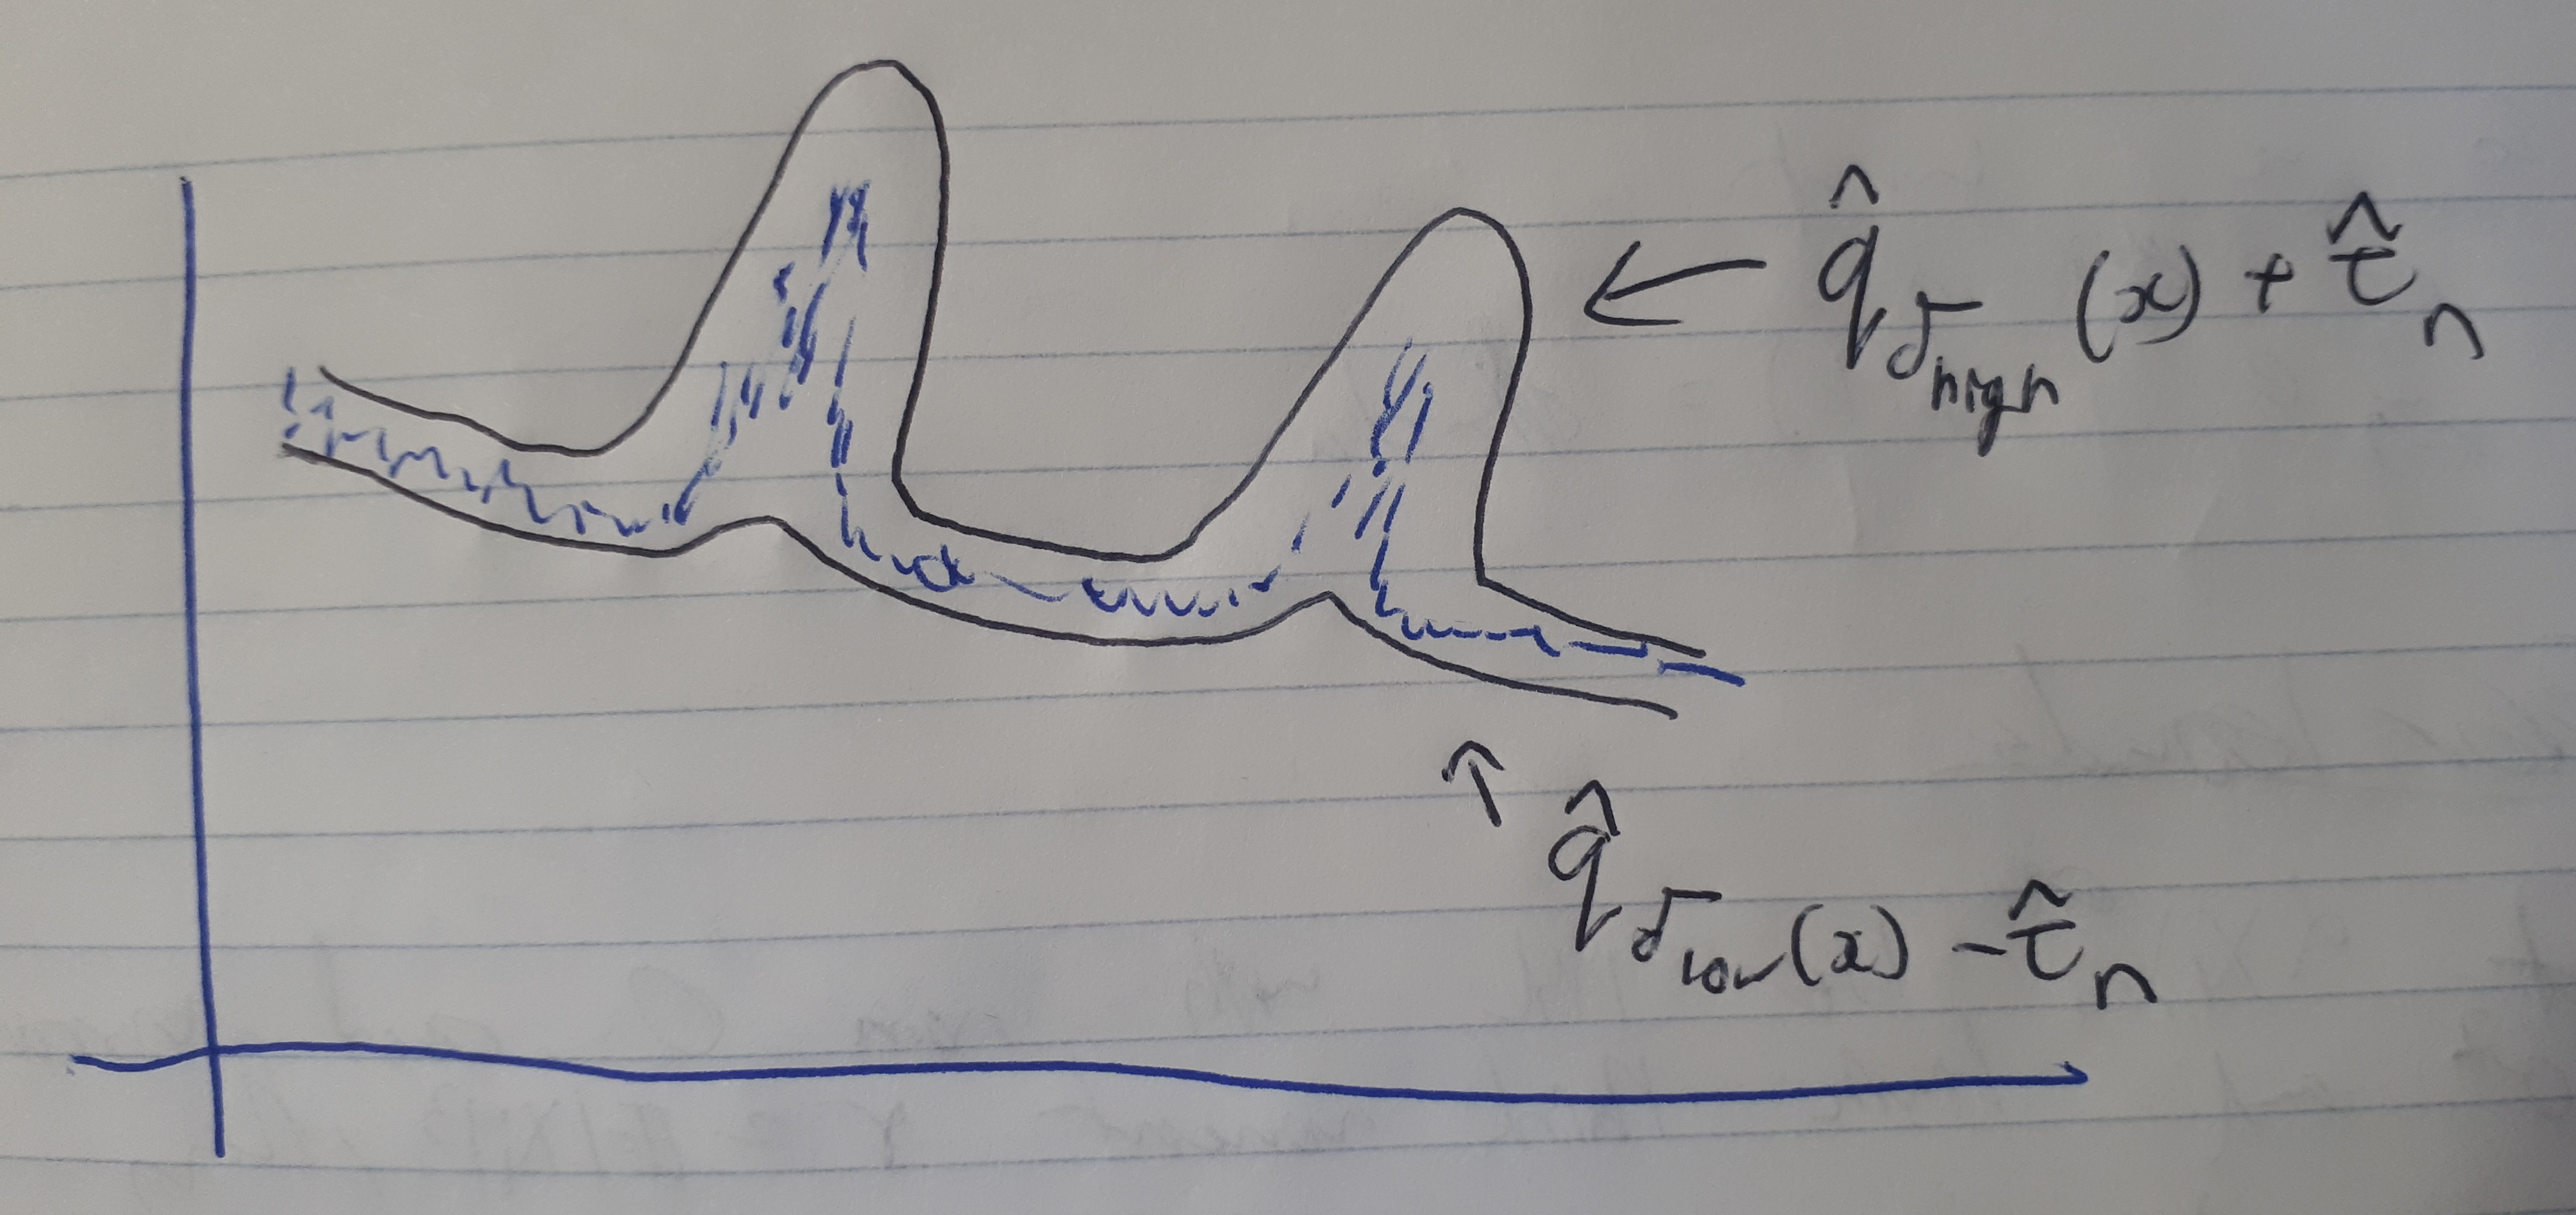
\includegraphics[width = 0.7\textwidth]{12_02_P04.jpg}
    \end{center}
\end{ex}
\section{Class summary}
People use models $Y=f(X) + \eps$. If we make assumptions on $f$ and $\eps$, then we can prove analytic results. If we do not want to make assumptions, we have to do some sort of validation.
\end{document}